\documentclass{standalone}

\usepackage{tikz}
\usetikzlibrary{arrows}
\usetikzlibrary{decorations.markings}

\begin{document}

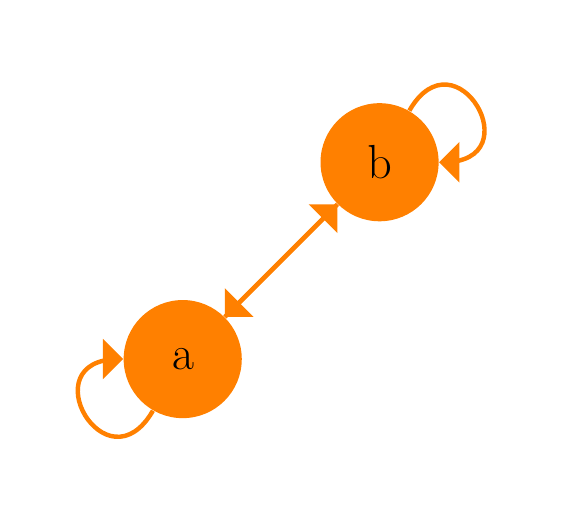
\begin{tikzpicture}
  \node (a) [style={minimum size=1.5cm,fill=orange,text=black,shape=circle}] at (0, 0) {\LARGE{a}};
  \node (b) [style={minimum size=1.5cm,fill=orange,text=black,shape=circle}] at (2.5, 2.5) {\LARGE{b}};

  \draw[draw=orange, ultra thick, -triangle 90] (a) -- (b);
  \draw[draw=orange, ultra thick, -triangle 90] (b) -- (a);

  \draw[draw=orange, ultra thick, -triangle 90] (a) to [out=-120,in=180,looseness=4] (a);

  \draw[draw=orange, ultra thick, -triangle 90] (b) to [out=-300,in=0,looseness=4] (b);

\end{tikzpicture}

\end{document}
